\chapter{Code Style}
Voor de code style worden de standaard code style settings van IntelliJ IDEA gebruikt.
De code style wordt ook gecontroleerd door Codacy, een code analyse tool.
Codacy controleert je Java (en Javascript) codebase op verschillende errors.

\begin{figure}[H]
	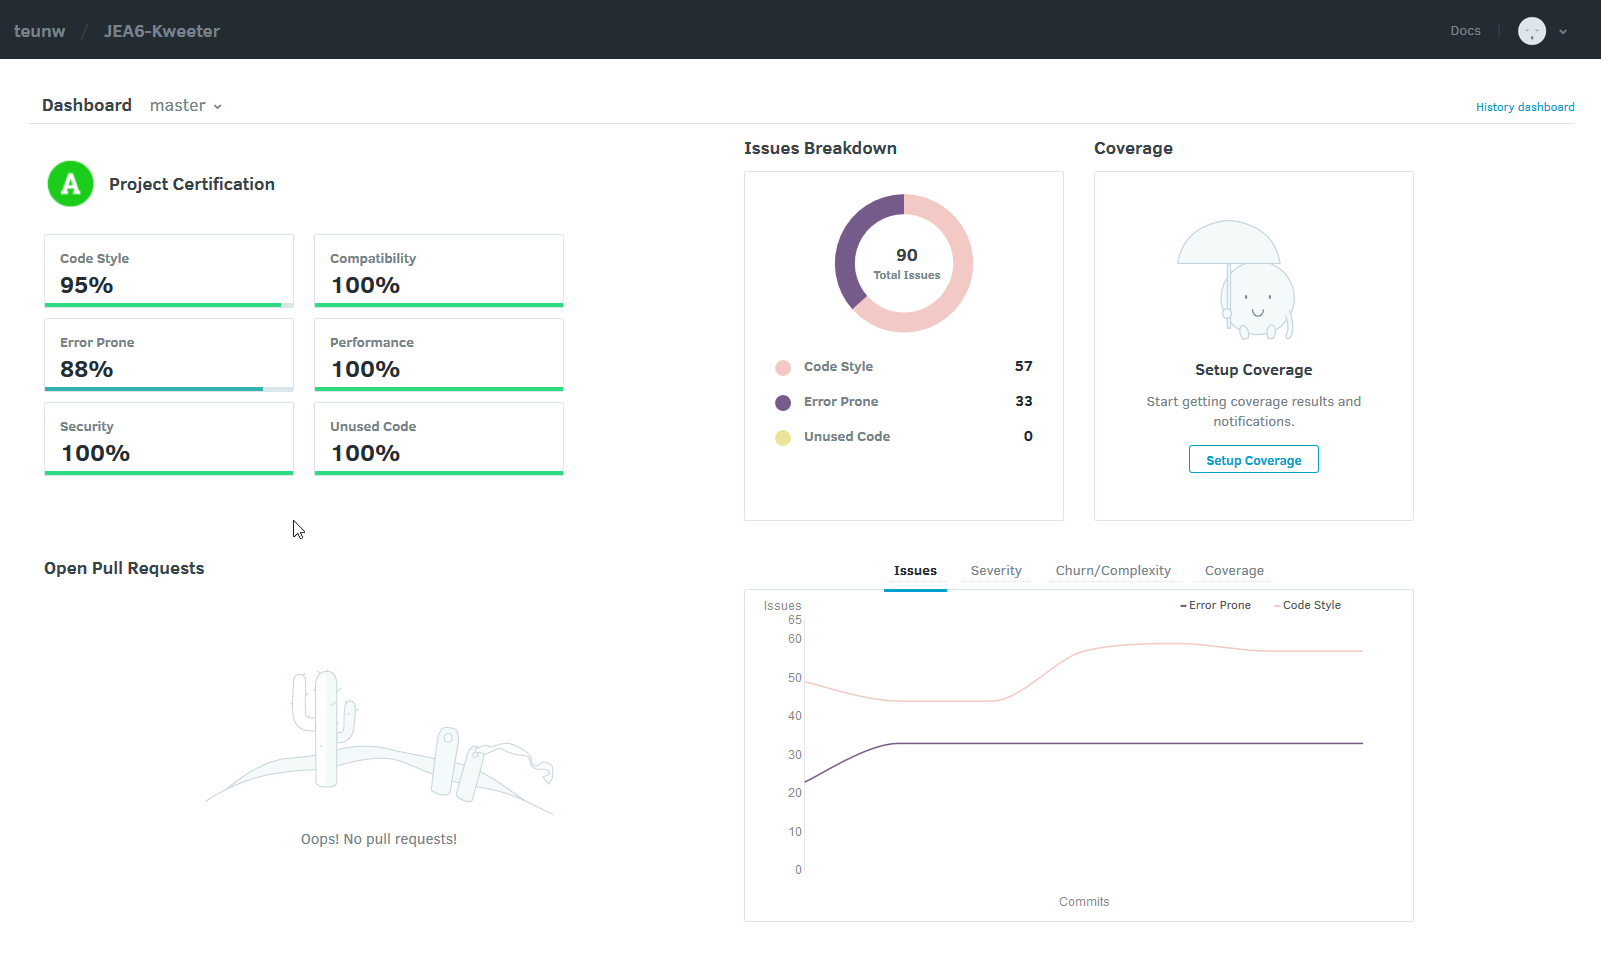
\includegraphics[width=0.75\textwidth]{images/StaticCodeAnalysis.png}
	\caption{Voorbeeld van code analysis door middel van Codacy}
	\label{fig:StaticCodeAnalyses}
\end{figure}

Ook kan er gecontroleerd worden op beveiligingsproblemen in je applicatie, stel dat je bijvoorbeeld SQL-query parameters in je queries hebt staan.

